%%%% 第一版 2020.10
%此文档为普通物理实验三林伟华老师要求的物理实验报告模板
%作者:武汉大学物理科学与技术学院18级詹睿知
%参考自电子信息学院实验报告模板
%%%% 第二版 2022.8
%更改优化了documentclass
\documentclass{WHUReport}
\usepackage[]{amsmath}
\usepackage{natbib}
\setcitestyle{numbers,square}
\usepackage{diagbox} %斜线表头

%%%% 以下填写学生信息及实验题目
\newcommand{\major}{物理学}
\newcommand{\name}{郑卜凡}
\newcommand{\stuid}{2021302022016}
\newcommand{\Name}{Bufan Zheng}
\newcommand{\course}{普通物理实验三}
\newcommand{\newtitle}{电子荷质比的测定}
\newcommand{\Title}{Determining the Charge-to-Mass Ratio of the Electron
}

\begin{document}
\pagestyle{maincontent} 
%\bibliographystyle{plain}

\begin{center}
\zihao{-2} \textbf{\newtitle}\\
\zihao{7}~\\
\zihao{4} \kaishu \name \ \ (\stuid)\\
\zihao{5} \kaishu (武汉大学物理科学与技术学院,湖北省 武汉市 430072)\\
\end{center}
\zihao{-5}\textbf{摘\quad 要:}
%在此处修改中文摘要
本实验利用磁聚焦法测量电子荷质比,最终与国际推荐测量值相对误差控制在$10\%$以内。利用Mathematica软件建模重现了实验螺线管内电子束的磁聚焦运动轨迹。本实验还分析了误差原因并给出了实验不确定度的估计。\\
\zihao{-5}\textbf{关键词:}电子;荷质比;磁聚焦;Mathematica
~\\
\begin{center}
	\zihao{3}\textbf{\Title}\\
	\zihao{-4} \Name\quad (\stuid)\\
	\zihao{5} School of physical science and technology, Wuhan University, Wuhan, 430072, China
\end{center}

\zihao{5}\textbf{Abstract:}In this paper, experimenters use the magnetic focusing method to determine the charge-to-mass ratio of electrons. Relative error from internationally recommended measurements was controlled about $10\%$. Using Mathematica software, the track of the electron beam in the solenoid was pictured. The experimental error and uncertainty also been presented.

\zihao{5}\textbf{Keywords: }electron; charge to mass ratio; magnetic focusing; Mathematica

\begin{multicols}{2}
	电子荷质比是一个非常重要的基本物理学量,与电子磁矩密切相关,所以在塞曼效应等与磁场有关的量子现象中电子荷质比参数与实验结果紧密相连。目前实验上有不少测量电子荷质比的实验手段,历史上最早的测量方法是汤姆孙利用电子在点场作用下偏转的特性给出的,后来还有比质谱仪法、双电容法\upcite{ref1},作为普通物理实验,还可以利用塞曼效应\upcite{ref2,ref6}、法拉第效应\upcite{ref3}、电解水\upcite{ref4}等进行测量。本次实验使用磁聚焦法\upcite{ref5}进行测量,优点是原理简单,测量方法容易掌握,而且误差相对较小。
	\section{实验原理}
	长直螺线管内部的磁场可近似看成均匀的轴向磁场,磁感应强度可用下式计算:
	\begin{equation}
		B=\frac{\mu_0 N I}{\sqrt{L^2+D_0^2}}
	\end{equation}
	其中$\mu_0$为真空磁导率,$I$为螺线管电流强度,$N$为匝数,$L$为螺线管长度,$D_0$为螺线管直径。
	
	实验装置首先通过加速电场给电子束中电子相同的轴向初速度$V_\parallel $:
	\begin{equation}
		V_{\parallel }=\sqrt{\frac{2e U}{m}}
	\end{equation}
	
	由于螺线管中的磁场是轴向的,所以如果没有给电子束加偏转电压,电子束不会被磁场偏转,这时在示波器上会看到一个亮点。现在给电子束加上偏转的交变电压,这会让电子束中的电子虽然从螺线管的同一位置出发,但是具有不同的横向速度$V_\perp$。横向速度会受到洛伦兹力的偏转从而具有一个向心的加速度,而轴向速度仍然不变,所以最终电子的运动是轴向的匀速直线运动与垂直于轴向平面内的匀速圆周运动的叠加。其中圆周运动的半径为:
	\begin{equation}
		R=\frac{mV_\perp}{e B}
	\end{equation}
	周期为:
	\begin{equation}
		T=\frac{2\pi R}{V_\perp}=\frac{2\pi m}{eB}
	\end{equation}
	在空间上看运动轨迹是一条螺旋线,螺距为:
	\begin{equation}
		h=V_\parallel T=\frac{2\pi}{B}\sqrt{\frac{2mU}{e}}
	\end{equation}
	
	从上式可以看出,电子做圆周运动的周期和螺距均与$V_\perp$无关。所以尽管电子的$V_\perp$不同,在一个周期过后,它们都会在一个相同的螺距处再次相遇。所以我们只需要调节电流,从而调节螺线管内磁感应强度,使得电子束运动的螺距恰好为起点到荧光屏的距离,我们便可以在荧光屏上再次看到一个亮点,即聚焦现象。电子的荷质比便由下式给出:
	\begin{equation}
		\frac{e}{m}=\frac{8\pi^2 U\left(L^2+D_0^2\right)^2}{\left(\mu_0 NIh\right)^2}
	\end{equation}
	
	 不难想象,实验上我们在加速电压$U$一定时调节励磁电流$I$,初始时会在荧光屏上看到一条亮线,表示磁场还未加入,交变偏转电压使得电子束分散。慢慢加大电流,亮线越来越短,表示电子束开始聚焦,而且因为磁场偏转,亮线会同时旋转。最终我们会在屏幕上看到第一个亮点,这说明此时荧光屏位置为一倍螺距。后面继续加大电压会看到第$N$个两点,说明荧光屏位置为$N$倍螺距。
	\section{Mathematica仿真}
	利用Mathematica可以绘制得到单个电子的运动轨迹:
	\begin{figure}[H]
		\centering
		\subfigure[正视图]{
			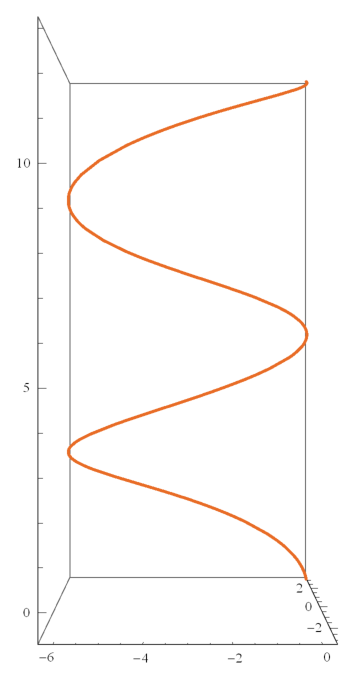
\includegraphics[width=0.48\linewidth]{./figs/1.eps}}
		\subfigure[缺省图]{
			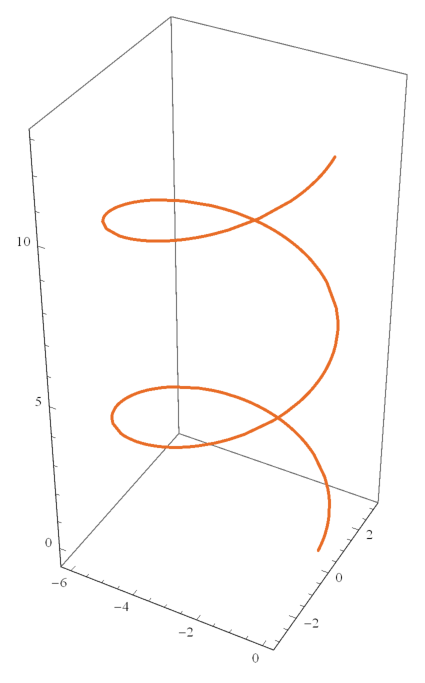
\includegraphics[width=0.48\linewidth]{./figs/3.eps}}
		\\
		\subfigure[俯视图]{
			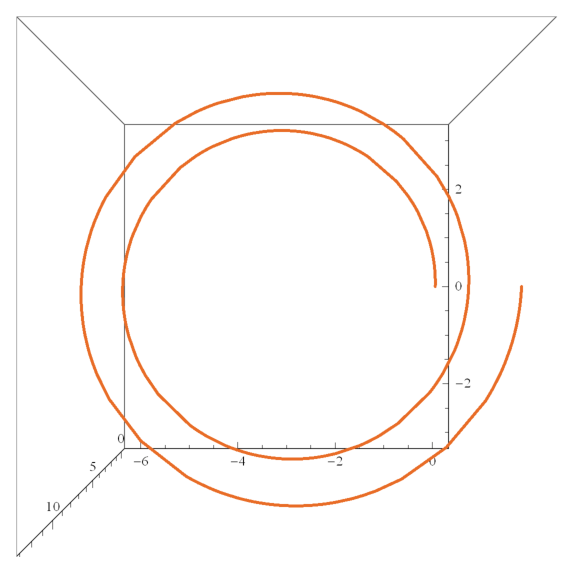
\includegraphics[width=0.48\linewidth]{./figs/2.eps}}
		\caption{单个电子的运动轨迹模拟,图中绘制了两个周期,注意绘图时遵循了近大远小原则。}
	\end{figure}
	\noindent{可以看到确实为螺旋线。}
	
	现在对多个电子的情况进行模拟,得到结果为:
	\begin{figure}[H]
		\centering
		\subfigure[正视图]{
			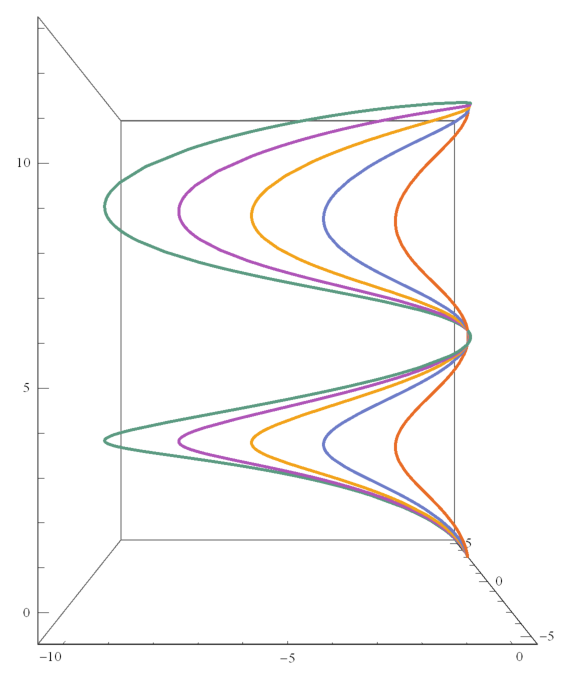
\includegraphics[width=0.48\linewidth]{./figs/4.eps}}
		\subfigure[俯视图]{
			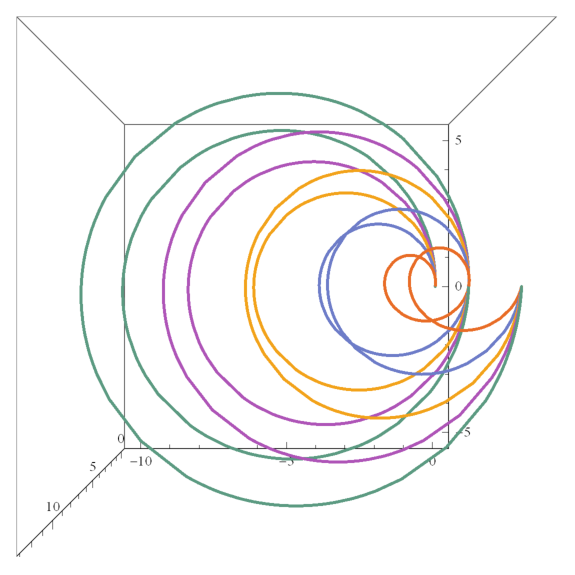
\includegraphics[width=0.48\linewidth]{./figs/5.eps}}
		\\
		\subfigure[缺省图]{
			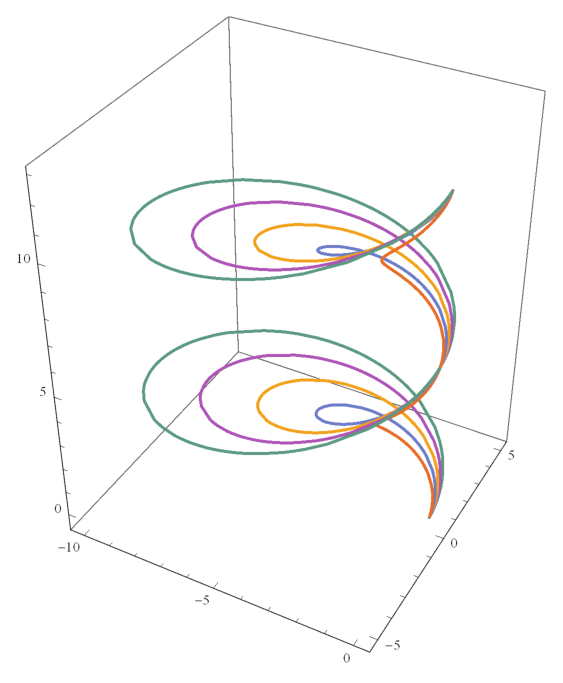
\includegraphics[width=0.48\linewidth]{./figs/6.eps}}
		\caption{多个电子的运动轨迹模拟,图中绘制了两个周期,注意绘图时同样遵循了近大远小原则。}
	\end{figure}
	\noindent{确实在螺距观察到了磁聚焦现象。}
	\section{实验步骤与数据}
	\subsection{实验步骤}
	
	按照前面的实验原理,按照下面的实验步骤进行实验:
	\begin{itemize}
		\item[1] 开启电子束测试仪电源开关,“电子束——荷质比”开关置于荷质比方向,此时荧光屏上出现一条直线;
		\item[2] 将励磁电流的调节旋钮逆时针方向调节到头,并将励磁电流输出与励磁电流输入相连;
		\item[3] 电流换向开关打向正向,调节输出调节旋钮,逐渐加大电流使荧光屏上的直线一边缩短一边旋转,直到出现第一个小光点,读取此时的电流值$I_{\text{正}}$,然后将电流调为0,再将电流换向开关打向反向,重复前面的过程得到$I_{\text{反}}$;
		\item[4] 改变阳极电压,重复前面的步骤测量多组数据。
	\end{itemize}
	\subsection{实验数据}
	实验数据如下表:
	\begin{table}[H]
		\scalebox{0.9}{
		\begin{tabular}{|c|c|c|c|c|}
			\hline
			\diagbox{励磁电流}{偏转电压}& 700V  & 800V  & 900V  & 1000V \\ \hline
			$I_{\text{正}}$(A) & 1.490 & 1.590 & 1.700 & 1.790 \\ \hline
			$I_{\text{正}}$(A) & 1.490 & 1.580 & 1.690 & 1.780 \\ \hline
			$\bar I$(A)       & 1.490 & 1.585 & 1.695 & 1.785 \\ \hline
			$e/m$($\times 10^{11}$C/kg)       & 1.925 & 1.944 &1.912 & 1.916 \\ \hline
		\end{tabular}
	}
	\end{table}
	其中荷质比的计算所用到的仪器参数为:
	\begin{itemize}
		\item[1] 匝数$N=535\pm 1$
		\item[2] 螺线管长度$L=0.235\operatorname{m}$
		\item[3] 螺线管直径$D_0=0.092\operatorname{m}$
		\item[4] 螺距(偏转版到荧光屏距离)$h=0.135\operatorname{m}$
	\end{itemize}
	\section{实验数据处理与误差分析}
	查阅文献\upcite{ref7,ref8}得知,不确定度可以用下式计算:
	\begin{equation}
		\begin{aligned}
			u^2(\frac{e}{m})/\bar{\left(\frac{e}{m}\right)}^2=&\left(\frac{u(U)}{U}\right)^2+\left(\frac{2u(h)}{h}\right)^2+\left(\frac{2u(I)}{I}\right)^2\\&+\left(\frac{u(N)}{N}\right)^2+\left(\frac{u(D_0)\cdot 2D_0}{L^2+D_0^2}\right)^2\\&+\left(\frac{u(L)\cdot 2L}{L^2+D_0^2}\right)^2
		\end{aligned}
	\end{equation}
	
	按照实验仪器提供的参数,$N$、$L$、$h$、$D_0$的不确定度分别为:$u(N)=1/\sqrt{3}$,$u(L)=u(h)=u(D_0)=0.001/\sqrt{3}$。实验中使用的加速电压由稳压电源提供,电压的随机误差可以忽略,主要以B类不确定度为主,可以取为$u=10/\sqrt{3}$。电流的B类不确定度由仪器引起的部分可以忽略,主要是因为聚焦点不易掌握引起的,可以取为$u_B(I)=0.01/\sqrt{3}$。本次实验属于等精度的多次测量,A类不确定度由标准差的平均值得到即$u_A=s/\sqrt{n}$,根据实验数据得知$u_A(I)=0.00375$所以电流的合成不确定度为$u(I)\approx 0.007$。代入不确定度计算公式最终得到:
	\begin{equation}
		u(e/m)\approx 0.016\times 10^{11} \operatorname{C/kg}
	\end{equation}
	所以最终测量结果表达为:
	\begin{equation}
		\frac{e}{m}=\left(1.924\pm0.016\right)\times 10^{11} \operatorname{C/kg}
	\end{equation}
	国际推荐测量值为$1.758\times 10^11$,相对误差为$9.4\%<10\%$。作为教学实验已经算是不错的结果,而且不确定度也比较小,可信度高。
	
	\subsection{误差原因分析}
	从不确定度公式可以看出,励磁电流测量的不确定度占有很大的比重,而聚焦点又并不太好掌握,所以这是引起误差的主要原因。另外,仪器本身的精度不够也占很大比重,而且电子本身之间存在斥力,会导致电子束之间扩张,从而产生误差,这是实验原理本身的缺陷。最后我们还可以估算一下螺线管中磁感应强度大小,取$I=2\operatorname{A}$:
	\begin{equation}
		B=\frac{\mu_0 N I}{\sqrt{L^2+D_0^2}}\approx 5.328\times 10^{-3}\operatorname{T}
	\end{equation}
	地磁场的量级在$10^{-5}\operatorname{T}$量级,对本实验有微小的影响。
	\section{结\quad 论}
	本次实验利用磁聚焦法测量了电子荷质比,并给出了不确定度,最终结果与真值相对误差小于$10\%$,实验完成的比较好。而且利用Mathematica建模直观地认识了螺线管中电子束的运动过程,更清晰地理解了实验原理。
	\bibliographystyle{unsrt}
	\begin{thebibliography}{99}  
		\bibitem{ref1}黄国龙.带电粒子荷质比的测量方法[J].中学物理教学参考,2002(11):33-35.
		\bibitem{ref2}邵先亦,杜达敏.从分裂波数差谈塞曼效应实验之电子荷质比的测量[J].大学物理实验,2019,32(06):47-52.
		\bibitem{ref3}王小怀,李卓凡.基于法拉第效应的电子荷质比测量及不确定度分析[J].大学物理实验,2010,23(03):65-68.
		\bibitem{ref4}刘光宇,郭利忠.用电解水法测量电子电荷和荷质比[J].河南科技,1989(Z1):43-44.
		\bibitem{ref5}尹社会,田睿.磁聚焦法测量电子荷质比实验现象分析[J].实验科学与技术,2014,12(02):1-3.
		\bibitem{ref6}刘志军.微机塞曼效应实验的改进和电子荷质比的编程测量[J].大学物理,2013,32(01):25-29.
		\bibitem{ref7}王琪,卢佃清,李新华.电子束实验仪测荷质比及其测量结果的不确定度评定[J].实验技术与管理,2006(02):26-28.
		\bibitem{ref8}刘晓薇.用磁聚焦法测量电子荷质比的误差分析[J].中国现代教育装备,2012(16):46-47.
	\end{thebibliography}
\end{multicols}

\end{document}
